%%%%%%%%%%%%%%%%%%%%%%%%%%%%%%%%%%%%%%%%%
% Jacobs Landscape Poster
% LaTeX Template
% Version 1.0 (29/03/13)
%
% Created by:
% Computational Physics and Biophysics Group, Jacobs University
% https://teamwork.jacobs-university.de:8443/confluence/display/CoPandBiG/LaTeX+Poster
% 
% Further modified by:
% Nathaniel Johnston (nathaniel@njohnston.ca)
%
% This template has been downloaded from:
% http://www.LaTeXTemplates.com
%
% License:
% CC BY-NC-SA 3.0 (http://creativecommons.org/licenses/by-nc-sa/3.0/)
%
%%%%%%%%%%%%%%%%%%%%%%%%%%%%%%%%%%%%%%%%%

%----------------------------------------------------------------------------------------
%	PACKAGES AND OTHER DOCUMENT CONFIGURATIONS
%----------------------------------------------------------------------------------------

\documentclass[final]{beamer}

\usepackage[scale=1.24]{beamerposter} % Use the beamerposter package for laying out the poster
\usepackage{hyperref}
\usetheme{confposter} % Use the confposter theme supplied with this template

\setbeamercolor{block title}{fg=ngreen,bg=white} % Colors of the block titles
\setbeamercolor{block body}{fg=black,bg=white} % Colors of the body of blocks
\setbeamercolor{block alerted title}{fg=white,bg=dblue!70} % Colors of the highlighted block titles
\setbeamercolor{block alerted body}{fg=black,bg=dblue!10} % Colors of the body of highlighted blocks
% Many more colors are available for use in beamerthemeconfposter.sty

%-----------------------------------------------------------
% Define the column widths and overall poster size
% To set effective sepwid, onecolwid and twocolwid values, first choose how many columns you want and how much separation you want between columns
% In this template, the separation width chosen is 0.024 of the paper width and a 4-column layout
% onecolwid should therefore be (1-(# of columns+1)*sepwid)/# of columns e.g. (1-(4+1)*0.024)/4 = 0.22
% Set twocolwid to be (2*onecolwid)+sepwid = 0.464
% Set threecolwid to be (3*onecolwid)+2*sepwid = 0.708

\newlength{\sepwid}
\newlength{\onecolwid}
\newlength{\twocolwid}
\newlength{\threecolwid}
\setlength{\paperwidth}{48in} % A0 width: 46.8in
\setlength{\paperheight}{36in} % A0 height: 33.1in
\setlength{\sepwid}{0.024\paperwidth} % Separation width (white space) between columns
\setlength{\onecolwid}{0.22\paperwidth} % Width of one column
\setlength{\twocolwid}{0.464\paperwidth} % Width of two columns
\setlength{\threecolwid}{0.708\paperwidth} % Width of three columns
\setlength{\topmargin}{-0.5in} % Reduce the top margin size
%-----------------------------------------------------------

\usepackage{graphicx}  % Required for including images

\usepackage{booktabs} % Top and bottom rules for tables

%----------------------------------------------------------------------------------------
%	TITLE SECTION 
%----------------------------------------------------------------------------------------

\title{Cloud Gateway} % Poster title

\author{Qianli Ma, Ayush Singh, Rahul Bahal and Mania Abdi} % Author(s)

\institute{College of Computer and Information Science, Northeastern University} % Institution(s)

%----------------------------------------------------------------------------------------

\begin{document}

\addtobeamertemplate{block end}{}{\vspace*{2ex}} % White space under blocks
\addtobeamertemplate{block alerted end}{}{\vspace*{2ex}} % White space under highlighted (alert) blocks

\setlength{\belowcaptionskip}{2ex} % White space under figures
\setlength\belowdisplayshortskip{2ex} % White space under equations

\begin{frame}[t] % The whole poster is enclosed in one beamer frame

\begin{columns}[t] % The whole poster consists of three major columns, the second of which is split into two columns twice - the [t] option aligns each column's content to the top

\begin{column}{\sepwid}\end{column} % Empty spacer column

\begin{column}{\onecolwid} % The first column

%----------------------------------------------------------------------------------------
%	OBJECTIVES
%----------------------------------------------------------------------------------------

\begin{alertblock}{Abstract}

Using Cloud gateway, we are proposing a cost effective hybrid cloud model to seamlessly expand resources on-demand.
\begin{itemize}
\item Provisioning resources for peak workloads is expensive.
\item Public Cloud resources are added to private cloud resources to provide more resources for peak workload.
\item All traffic flows from Public through the Private Cloud, secured using an IPsec tunnel protocol.
\end{itemize}

\end{alertblock}

%----------------------------------------------------------------------------------------
%	INTRODUCTION
%----------------------------------------------------------------------------------------

\begin{block}{Introduction}

\begin{itemize}
\item The average-sized workload stays in the private cloud, and peak workload is provided via public cloud burst.
\item Cloud Gateway provides the admin of private cloud seamless and secure integration between an organization\'s on-premises IT environment and cloud service providers.
\item Machines will utilize the CG to send traffic between the private and public cloud subnets.
\item Workers on public side communicates to internet via the cloud gateway on private side to ensure they follow the organization firewall rules.
\end{itemize}



\end{block}

%------------------------------------------------

\begin{figure}
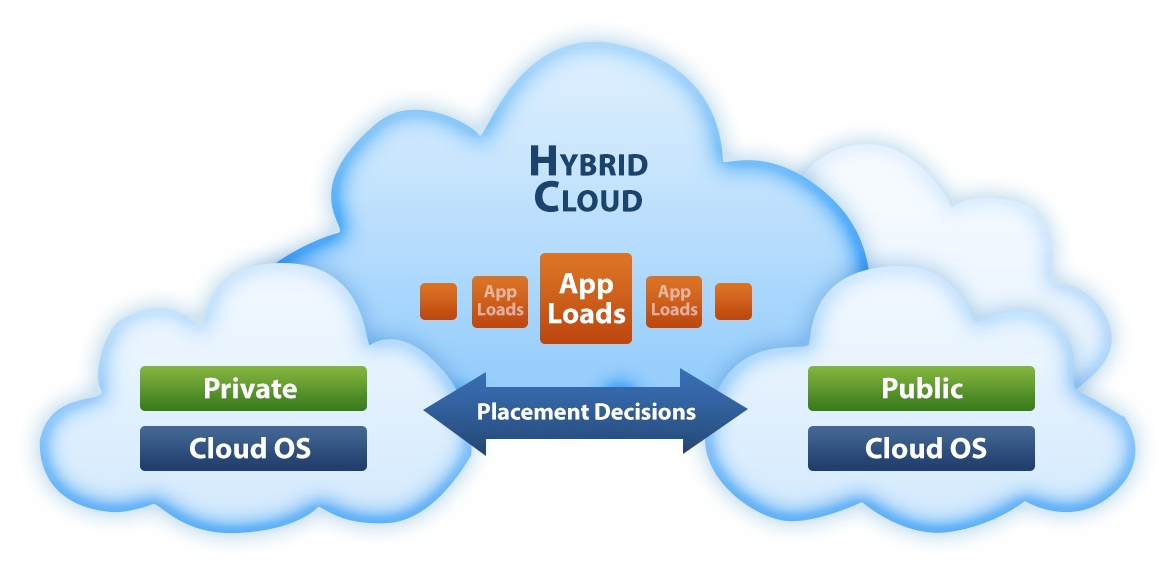
\includegraphics[width=0.8\linewidth]{bigpic.png}
\caption{Hybrid cloud using Cloud Gateway}
\end{figure}

%----------------------------------------------------------------------------------------

\end{column} % End of the first column

\begin{column}{\sepwid}\end{column} % Empty spacer column

\begin{column}{\twocolwid} % Begin a column which is two columns wide (column 2)

\begin{columns}[t,totalwidth=\twocolwid] % Split up the two columns wide column

\begin{column}{\onecolwid}\vspace{-.6in} % The first column within column 2 (column 2.1)

%----------------------------------------------------------------------------------------
%	MATERIALS
%----------------------------------------------------------------------------------------

\begin{block}{Architecture}

We designed an efficient architecture for expanding resources to withstand high workload.

\begin{itemize}
\item The data stream in private cloud is forwarded to cloud gateway.
\item The cloud gateway forwards the packet to private cloud by reforming IP header with gateway address.
\item Used iptables DNAT and Port forwarding to maintain consistent iptable in both public and private clouds.
\end{itemize}



\end{block}

%----------------------------------------------------------------------------------------

\end{column} % End of column 2.1

\begin{column}{\onecolwid}\vspace{-.6in} % The second column within column 2 (column 2.2)

%----------------------------------------------------------------------------------------
%	METHODS
%----------------------------------------------------------------------------------------

\begin{block}{User Interface}
User interface is used to configure cloud gateway.
\begin{itemize}
\item It exposes web service api, master-slave mode between VCG to faciliate control of network.
\item It is open source under Apache 2.0 License.
\item The webAPP allows the user to do DNAT, enable/disable internet and modify port forwarding tables.
\item It makes sure that IP tables on both virtual cloud gateways are consistent. 
\item It is written in Flask (Python) backend, sqlite3 database.
\end{itemize}

\end{block}

%----------------------------------------------------------------------------------------

\end{column} % End of column 2.2

\end{columns} % End of the split of column 2 - any content after this will now take up 2 columns width

%----------------------------------------------------------------------------------------
%	IMPORTANT RESULT
%----------------------------------------------------------------------------------------



%----------------------------------------------------------------------------------------

\begin{columns}[t,totalwidth=\twocolwid] % Split up the two columns wide column again

\begin{column}{\onecolwid} % The first column within column 2 (column 2.1)

%----------------------------------------------------------------------------------------
%	MATHEMATICAL SECTION
%----------------------------------------------------------------------------------------

\begin{block}{Cloud Configuration}

\begin{itemize}
\item We install CG assuming a virtual private cloud is already setup in an organization. 
\item A CloudFormation template which take some parameter to set up VPC, subnet, cloud gateway VM etc.
\item Amazon AWS and MOC OpenStack were used as test framework implying that the design is applicable to any cloud.
\begin{itemize}
\item Amazon AWS virtual gateway is setup with source/destination cheking disabled.
\item MOC OpenStack virtual gateway is configured with source/destination checking disabled.
\item Private virtual clouds are formed in different subnet from cloud gateway.
\item All data from virtual cloud are routed to cloud gateway.
\end{itemize}
\end{itemize}

\begin{figure}
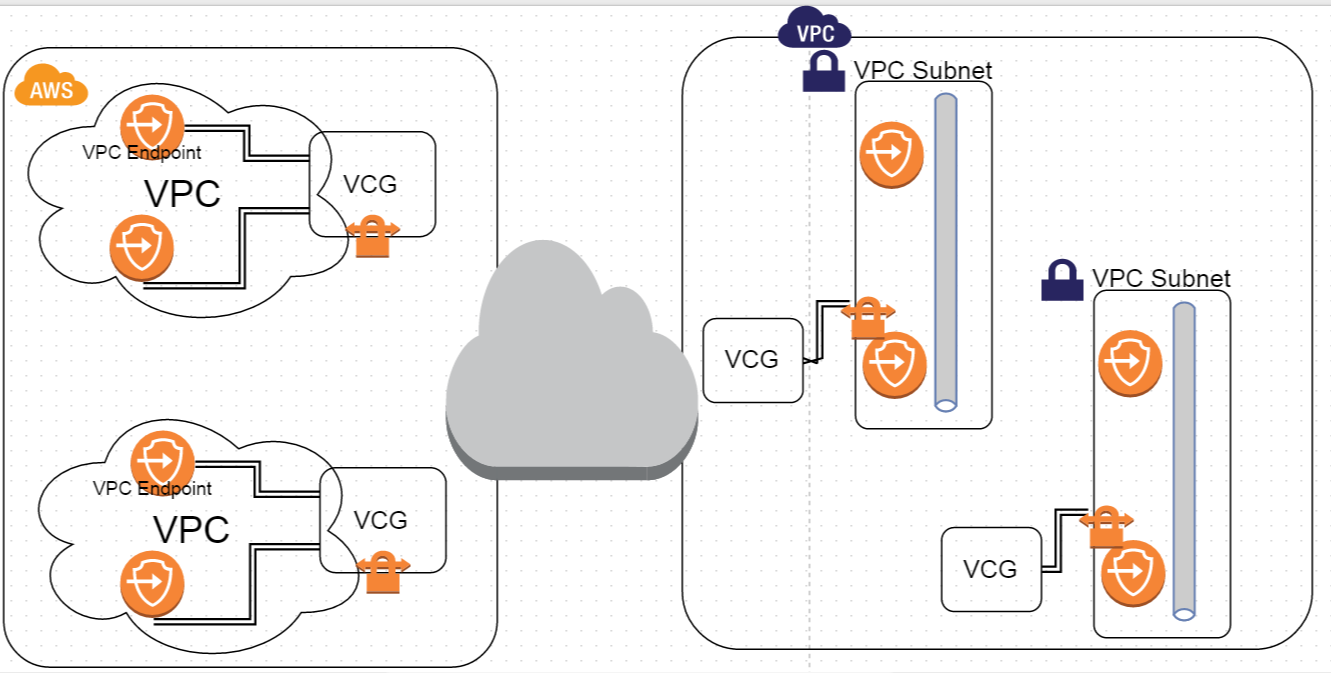
\includegraphics[width=0.8\linewidth]{connection.png}
\caption{Cloud Gateway Architecture}
\end{figure}

\end{block}

%----------------------------------------------------------------------------------------

\end{column} % End of column 2.1

\begin{column}{\onecolwid} % The second column within column 2 (column 2.2)

%----------------------------------------------------------------------------------------
%	RESULTS
%----------------------------------------------------------------------------------------

\begin{block}{Cloud Gateway Deliver}

\begin{figure}
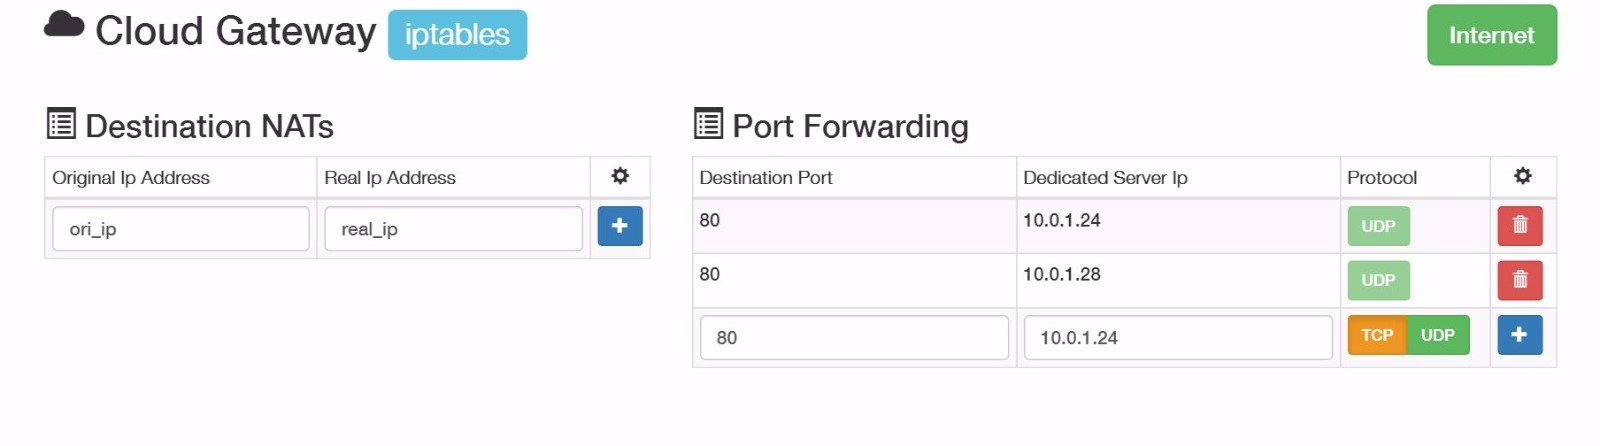
\includegraphics[width=0.8\linewidth]{interface.jpg}
\caption{User Interface}
\end{figure}


\begin{itemize}
\item Rests on private and scales on demand via cloud burst to Public Cloud.
\item Open source User-friendly interface to deal with configuration.
\item Open source console tools to configure public cloud and private cloud.
\item Cloud formation Templates to setup public cloud infrastructure.
\end{itemize}

\end{block}


%----------------------------------------------------------------------------------------

\end{column} % End of column 2.2

\end{columns} % End of the split of column 2

\end{column} % End of the second column

\begin{column}{\sepwid}\end{column} % Empty spacer column

\begin{column}{\onecolwid} % The third column


%----------------------------------------------------------------------------------------
%	CONCLUSION
%----------------------------------------------------------------------------------------


\begin{figure}
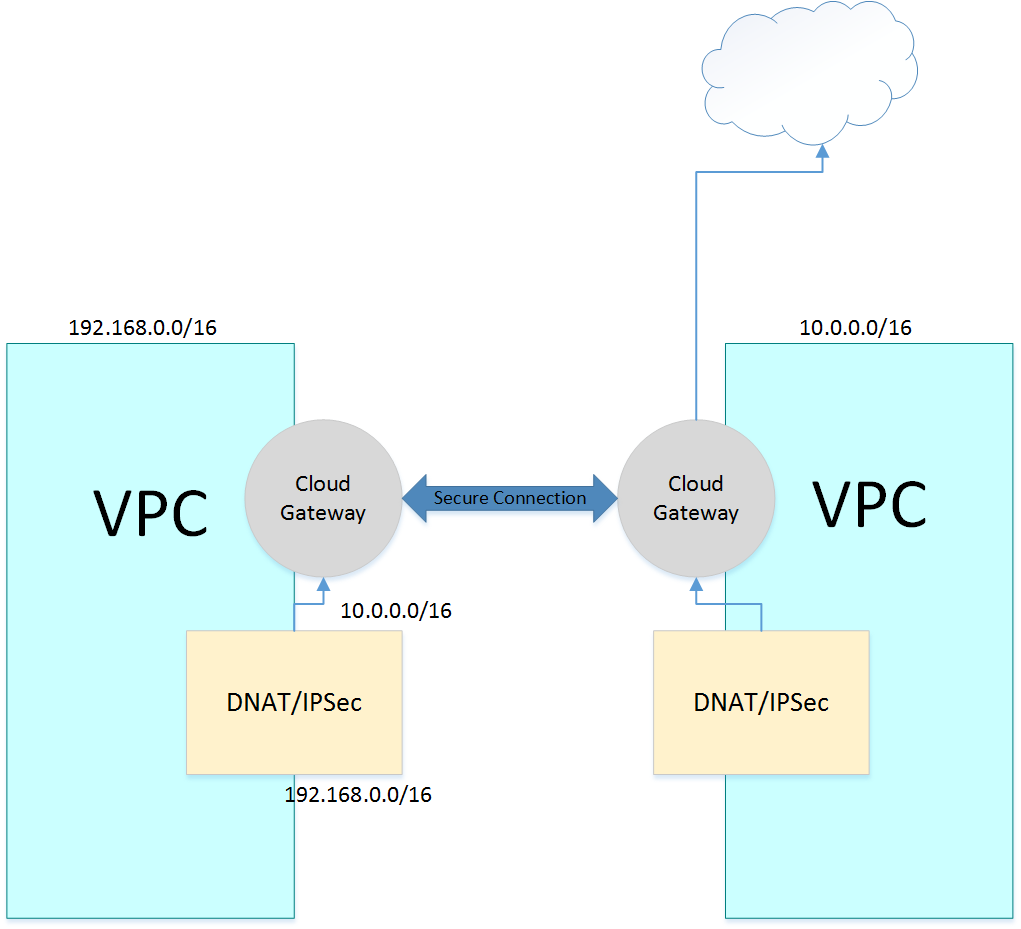
\includegraphics[width=0.8\linewidth]{Gatewayr.png}
\caption{Gateway Setup}
\end{figure}


\begin{block}{Conclusion}

\begin{itemize}
\item The hybrid cloud model is a cost-effective method.
\item The average-size workload stays in private cloud.
\item Machines use CG to send traffic b/w different cloud subnets.
\end{itemize}

\end{block}

%----------------------------------------------------------------------------------------
%	ADDITIONAL INFORMATION
%----------------------------------------------------------------------------------------



%----------------------------------------------------------------------------------------
%	REFERENCES
%----------------------------------------------------------------------------------------

\begin{block}{ACKNOWLEDGEMENTS}
Thanks to Kyle Forster and Ted Elhourani in BigSwitch. 
\end{block}

%----------------------------------------------------------------------------------------
%	ACKNOWLEDGEMENTS
%----------------------------------------------------------------------------------------



%----------------------------------------------------------------------------------------
%	CONTACT INFORMATION
%----------------------------------------------------------------------------------------

\setbeamercolor{block alerted title}{fg=black,bg=norange} % Change the alert block title colors
\setbeamercolor{block alerted body}{fg=black,bg=white} % Change the alert block body colors

\begin{alertblock}{Contact Information}

\begin{itemize}
\item \href{http://www.bu.edu/hic/research/massachusetts-open-cloud/}{Massachusetts Open Cloud}
\item \href{https://github.com/rahulbahal7/cloud-gateway}{Git Repository}
\end{itemize}

\end{alertblock}


%----------------------------------------------------------------------------------------

\end{column} % End of the third column

\end{columns} % End of all the columns in the poster

\end{frame} % End of the enclosing frame

\end{document}
